\documentclass[12pt,a4paper]{article}
\usepackage[utf8]{inputenc}
\usepackage[margin=1in]{geometry}
\usepackage{graphicx}
\usepackage{listings}
\usepackage{xcolor}
\usepackage{amsmath}
\usepackage{fancyhdr}
\usepackage{titlesec}
\usepackage{hyperref}
\usepackage{float}

% Code listing style
\definecolor{codegreen}{rgb}{0,0.6,0}
\definecolor{codegray}{rgb}{0.5,0.5,0.5}
\definecolor{codepurple}{rgb}{0.58,0,0.82}
\definecolor{backcolour}{rgb}{0.95,0.95,0.92}

\lstdefinestyle{mystyle}{
    backgroundcolor=\color{backcolour},   
    commentstyle=\color{codegreen},
    keywordstyle=\color{magenta},
    numberstyle=\tiny\color{codegray},
    stringstyle=\color{codepurple},
    basicstyle=\ttfamily\footnotesize,
    breakatwhitespace=false,         
    breaklines=true,                 
    captionpos=b,                    
    keepspaces=true,                 
    numbers=left,                    
    numbersep=5pt,                  
    showspaces=false,                
    showstringspaces=false,
    showtabs=false,                  
    tabsize=4
}
\lstset{style=mystyle}

% Header and Footer
\pagestyle{fancy}
\fancyhf{}
\rhead{Computer Graphics Lab}
\lhead{Lab 4}
\rfoot{Page \thepage}

\begin{document}

% Title Page
\begin{titlepage}
    \centering
    \vspace*{1cm}
    
    \Huge
    \textbf{Computer Graphics Laboratory}
    
    \vspace{0.5cm}
    \LARGE
    Lab Report 4
    
    \vspace{1.5cm}
    
    \Large
    \textbf{Line and Polygon Clipping Algorithms}
    
    \vspace{2cm}
    
    \textbf{Submitted By:}\\
    \vspace{0.3cm}
    \Large
    Student Name
    
    \vspace{2cm}
    
    \textbf{Date:}\\
    \vspace{0.3cm}
    \today
    
    \vfill
    
    \large
    Department of Computer Science\\
    5th Semester
    
\end{titlepage}

\tableofcontents
\newpage

%===========================================
% TASK 1: COHEN-SUTHERLAND LINE CLIPPING
%===========================================
\section{Cohen-Sutherland Line Clipping Algorithm}

\subsection{Title of Lab Activity}
Implementation of Cohen-Sutherland line clipping algorithm to clip lines against a rectangular window using region codes and divide-and-conquer approach.

\subsection{Algorithm used for drawing line}
Digital Differential Analyzer (DDA) and Bresenham's line algorithm are used for line rasterization after clipping. The Cohen-Sutherland algorithm determines which portions of lines lie within the clipping window before rendering.

\textbf{Cohen-Sutherland Algorithm Steps:}
\begin{enumerate}
    \item Define region codes for the clipping window:
    \begin{itemize}
        \item INSIDE = 0000, LEFT = 0001, RIGHT = 0010
        \item BOTTOM = 0100, TOP = 1000
    \end{itemize}
    \item Compute region codes for both endpoints of the line
    \item Test the line segment:
    \begin{itemize}
        \item If both codes are 0000: line is completely inside (accept)
        \item If logical AND of codes $\neq$ 0: line is completely outside (reject)
        \item Otherwise: line crosses boundary (divide and test)
    \end{itemize}
    \item For boundary crossing: compute intersection point and replace endpoint
    \item Repeat until line is accepted or rejected
\end{enumerate}

\subsection{Source Code}
\begin{lstlisting}[language=Python, caption=Cohen-Sutherland Line Clipping Implementation]
INSIDE, LEFT, RIGHT, BOTTOM, TOP = 0, 1, 2, 4, 8

def _compute_out_code(x: float, y: float, rect: Rect) -> int:
    code = INSIDE
    if x < rect.xmin:
        code |= LEFT
    elif x > rect.xmax:
        code |= RIGHT
    if y < rect.ymin:
        code |= BOTTOM
    elif y > rect.ymax:
        code |= TOP
    return code

def cohen_sutherland_clip(line: Line, rect: Rect) -> Optional[Line]:
    x1, y1, x2, y2 = line
    out_code1 = _compute_out_code(x1, y1, rect)
    out_code2 = _compute_out_code(x2, y2, rect)

    while True:
        if out_code1 == 0 and out_code2 == 0:
            return (x1, y1, x2, y2)  # Accept
        if out_code1 & out_code2:
            return None  # Reject

        out_code_out = out_code1 or out_code2

        # Calculate intersection point
        if out_code_out & TOP:
            x = x1 + (x2 - x1) * (rect.ymax - y1) / (y2 - y1)
            y = rect.ymax
        elif out_code_out & BOTTOM:
            x = x1 + (x2 - x1) * (rect.ymin - y1) / (y2 - y1)
            y = rect.ymin
        elif out_code_out & RIGHT:
            y = y1 + (y2 - y1) * (rect.xmax - x1) / (x2 - x1)
            x = rect.xmax
        else:
            y = y1 + (y2 - y1) * (rect.xmin - x1) / (x2 - x1)
            x = rect.xmin

        # Replace endpoint and update region code
        if out_code_out == out_code1:
            x1, y1 = x, y
            out_code1 = _compute_out_code(x1, y1, rect)
        else:
            x2, y2 = x, y
            out_code2 = _compute_out_code(x2, y2, rect)
\end{lstlisting}

\subsection{Output}
\begin{figure}[H]
    \centering
    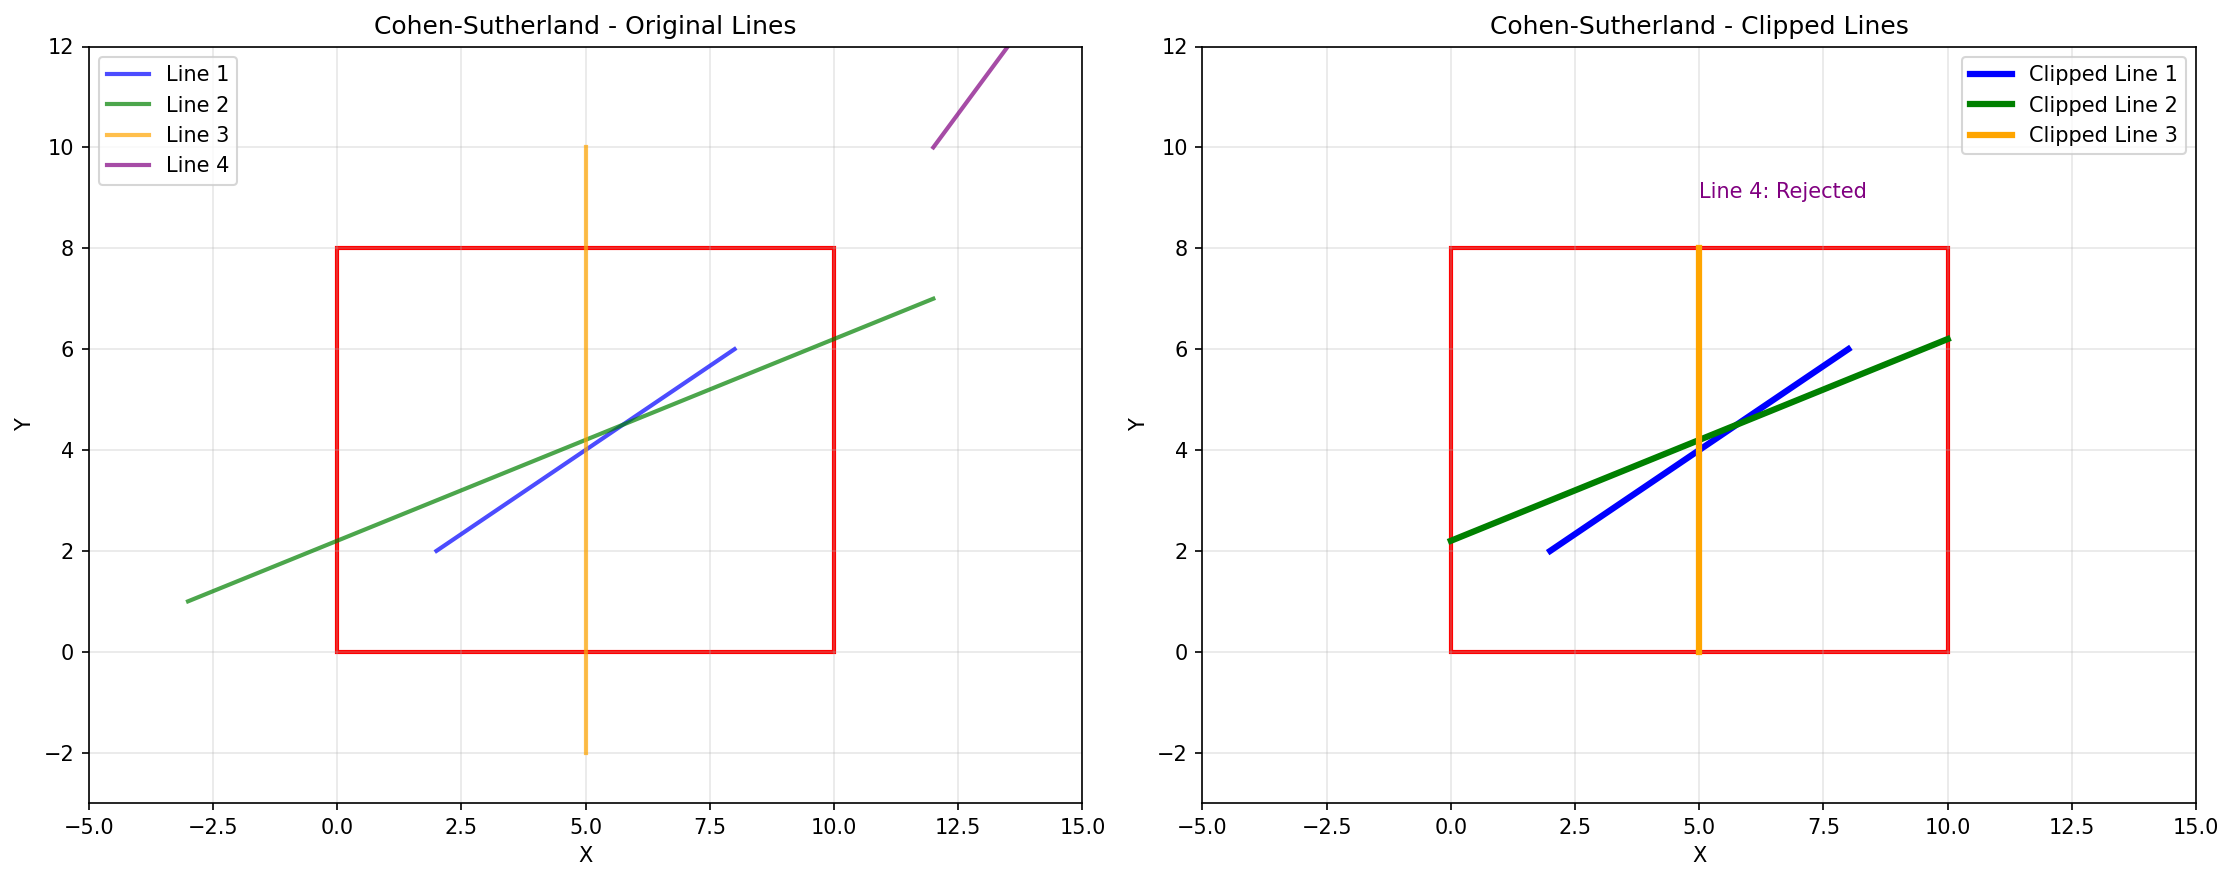
\includegraphics[width=0.8\textwidth]{output_cohen_sutherland.png}
    \caption{Cohen-Sutherland: Original lines vs Clipped lines within rectangular window}
\end{figure}

\newpage
%===========================================
% TASK 2: LIANG-BARSKY LINE CLIPPING
%===========================================
\section{Liang-Barsky Line Clipping Algorithm}

\subsection{Title of Lab Activity}
Implementation of Liang-Barsky line clipping algorithm using parametric line equations and efficient calculations to determine visible portions of lines within a rectangular window.

\subsection{Algorithm used for drawing line}
Digital Differential Analyzer (DDA) and Bresenham's line algorithm handle the actual line drawing after clipping. Liang-Barsky algorithm uses parametric representation for more efficient clipping calculations.

\textbf{Liang-Barsky Algorithm Steps:}
\begin{enumerate}
    \item Represent line parametrically: $P(t) = P_1 + t(P_2 - P_1)$ where $0 \leq t \leq 1$
    \item Define direction vector: $dx = x_2 - x_1$, $dy = y_2 - y_1$
    \item Set up inequality constraints for clipping window:
    \begin{itemize}
        \item $p_1 = -dx$, $q_1 = x_1 - x_{min}$ (left boundary)
        \item $p_2 = dx$, $q_2 = x_{max} - x_1$ (right boundary)
        \item $p_3 = -dy$, $q_3 = y_1 - y_{min}$ (bottom boundary)
        \item $p_4 = dy$, $q_4 = y_{max} - y_1$ (top boundary)
    \end{itemize}
    \item For each boundary, compute $u = -q_i / p_i$
    \item Update parameter range $[u_1, u_2]$ based on entering/leaving boundaries
    \item If $u_1 \leq u_2$: compute clipped endpoints, otherwise reject line
\end{enumerate}

\subsection{Source Code}
\begin{lstlisting}[language=Python, caption=Liang-Barsky Line Clipping Implementation]
def liang_barsky_clip(line: Line, rect: Rect) -> Optional[Line]:
    x1, y1, x2, y2 = line
    dx = x2 - x1
    dy = y2 - y1

    # Direction vectors and boundary distances
    p = [-dx, dx, -dy, dy]
    q = [x1 - rect.xmin, rect.xmax - x1, y1 - rect.ymin, rect.ymax - y1]

    u1, u2 = 0.0, 1.0
    
    for pk, qk in zip(p, q):
        if pk == 0:
            if qk < 0:
                return None  # Line parallel to boundary and outside
            continue
        
        u = -qk / pk
        
        if pk < 0:  # Entering boundary
            if u > u2:
                return None
            if u > u1:
                u1 = u
        else:  # Leaving boundary
            if u < u1:
                return None
            if u < u2:
                u2 = u

    # Calculate clipped endpoints using parameter values
    clipped_start = (x1 + u1 * dx, y1 + u1 * dy)
    clipped_end = (x1 + u2 * dx, y1 + u2 * dy)
    return (*clipped_start, *clipped_end)
\end{lstlisting}

\subsection{Output}
\begin{figure}[H]
    \centering
    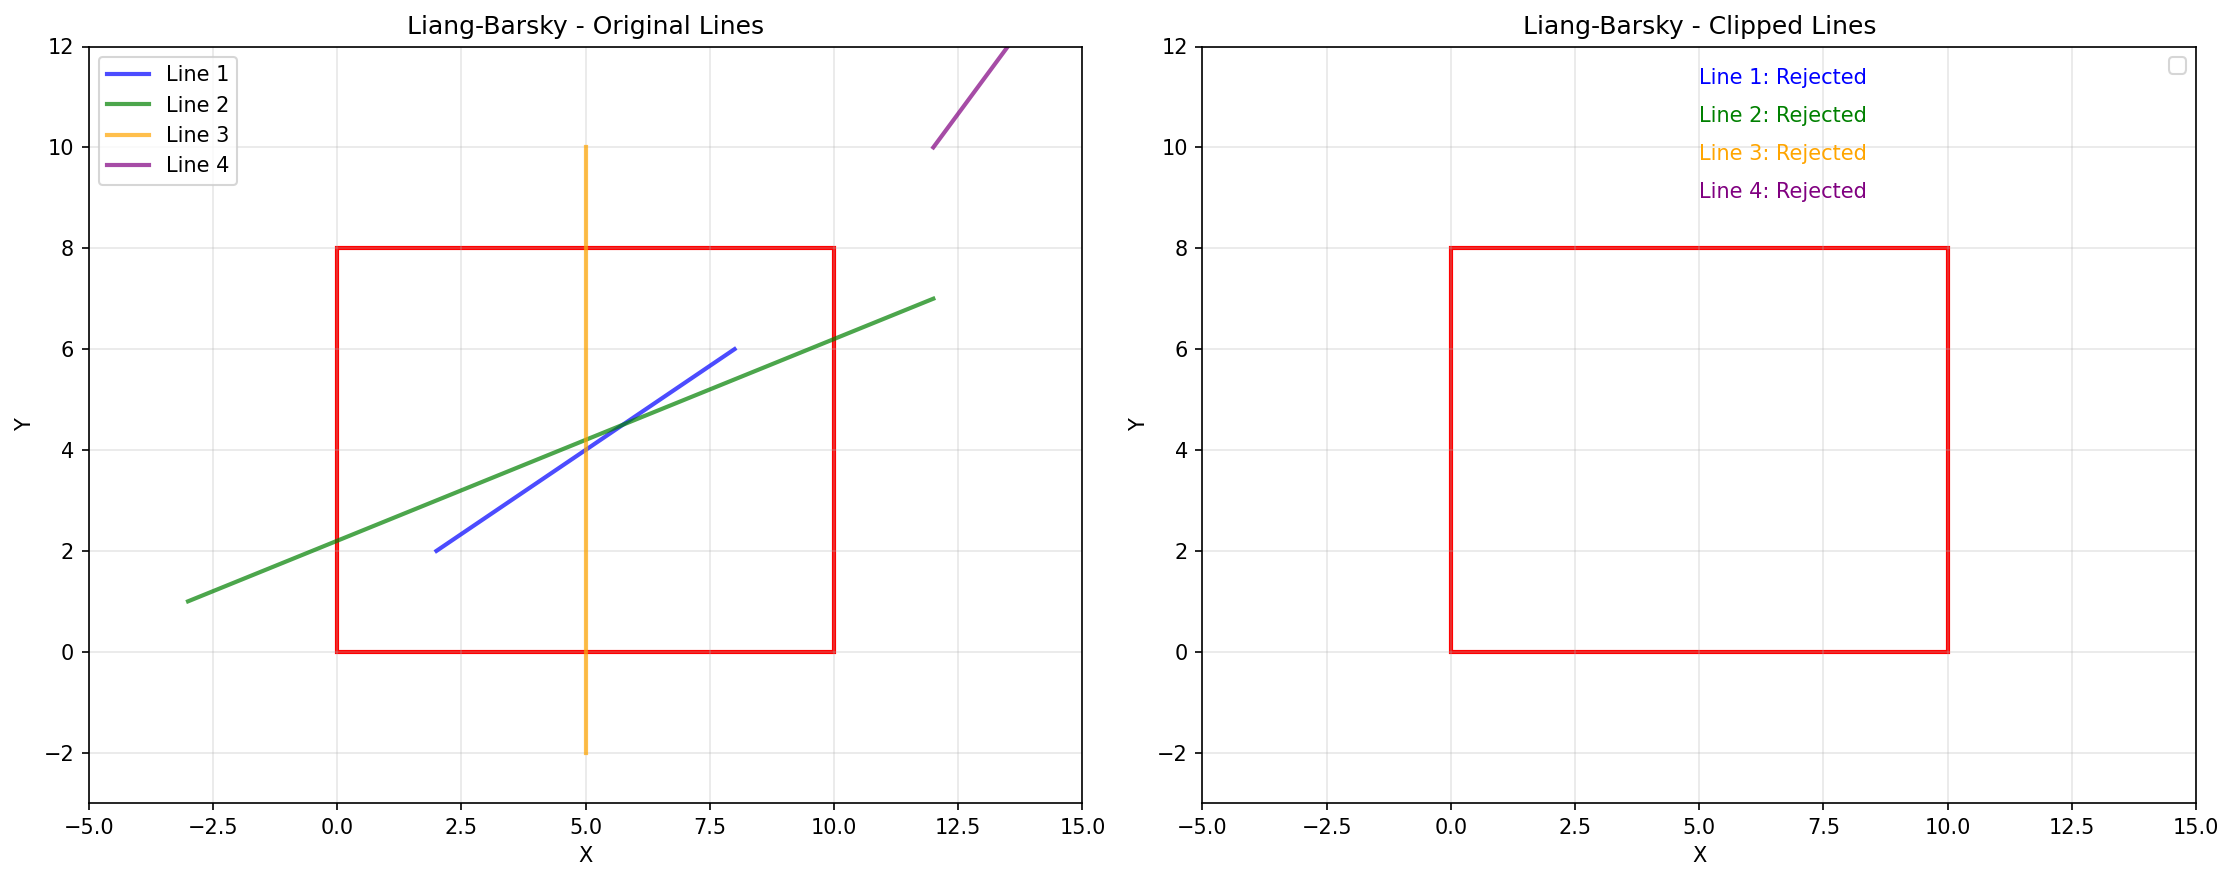
\includegraphics[width=0.8\textwidth]{output_liang_barsky.png}
    \caption{Liang-Barsky: Original lines vs Clipped lines using parametric approach}
\end{figure}

\newpage
%===========================================
% TASK 3: SUTHERLAND-HODGMAN POLYGON CLIPPING
%===========================================
\section{Sutherland-Hodgman Polygon Clipping Algorithm}

\subsection{Title of Lab Activity}
Implementation of Sutherland-Hodgman polygon clipping algorithm to clip convex polygons against convex clipping windows using successive edge clipping approach.

\subsection{Algorithm used for drawing line}
Digital Differential Analyzer (DDA) and Bresenham's line algorithm are used for drawing the clipped polygon edges. The Sutherland-Hodgman algorithm processes polygon vertices sequentially against each clipping edge.

\textbf{Sutherland-Hodgman Algorithm Steps:}
\begin{enumerate}
    \item Start with input polygon vertices
    \item For each edge of the clipping window:
    \begin{itemize}
        \item Process all vertices of current polygon
        \item For each edge of subject polygon, determine relationship to clip edge
    \end{itemize}
    \item For each polygon edge $(s, e)$:
    \begin{itemize}
        \item Case 1: Both inside → output $e$
        \item Case 2: $s$ inside, $e$ outside → output intersection
        \item Case 3: Both outside → output nothing
        \item Case 4: $s$ outside, $e$ inside → output intersection and $e$
    \end{itemize}
    \item Result from one clip edge becomes input for next clip edge
    \item Final result is the clipped polygon
\end{enumerate}

\subsection{Source Code}
\begin{lstlisting}[language=Python, caption=Sutherland-Hodgman Polygon Clipping Implementation]
def _is_inside(point: Point, edge_start: Point, edge_end: Point) -> bool:
    x, y = point
    x1, y1 = edge_start
    x2, y2 = edge_end
    # Check if point is on inside side of directed edge
    return (x2 - x1) * (y - y1) - (y2 - y1) * (x - x1) >= 0

def _compute_intersection(p1: Point, p2: Point, c1: Point, c2: Point) -> Point:
    x1, y1 = p1
    x2, y2 = p2
    x3, y3 = c1
    x4, y4 = c2

    denom = (x1 - x2) * (y3 - y4) - (y1 - y2) * (x3 - x4)
    if denom == 0:
        return p2

    px = ((x1 * y2 - y1 * x2) * (x3 - x4) - (x1 - x2) * (x3 * y4 - y3 * x4)) / denom
    py = ((x1 * y2 - y1 * x2) * (y3 - y4) - (y1 - y2) * (x3 * y4 - y3 * x4)) / denom
    return (px, py)

def sutherland_hodgman_clip(subject_polygon, clip_polygon):
    output_list = list(subject_polygon)
    if not output_list:
        return []

    clip_points = list(clip_polygon)
    for i in range(len(clip_points)):
        input_list = output_list
        output_list = []
        c_start = clip_points[i]
        c_end = clip_points[(i + 1) % len(clip_points)]

        if not input_list:
            break

        s = input_list[-1]
        for e in input_list:
            if _is_inside(e, c_start, c_end):
                if not _is_inside(s, c_start, c_end):
                    output_list.append(_compute_intersection(s, e, c_start, c_end))
                output_list.append(e)
            elif _is_inside(s, c_start, c_end):
                output_list.append(_compute_intersection(s, e, c_start, c_end))
            s = e
    return output_list
\end{lstlisting}

\subsection{Output}
\begin{figure}[H]
    \centering
    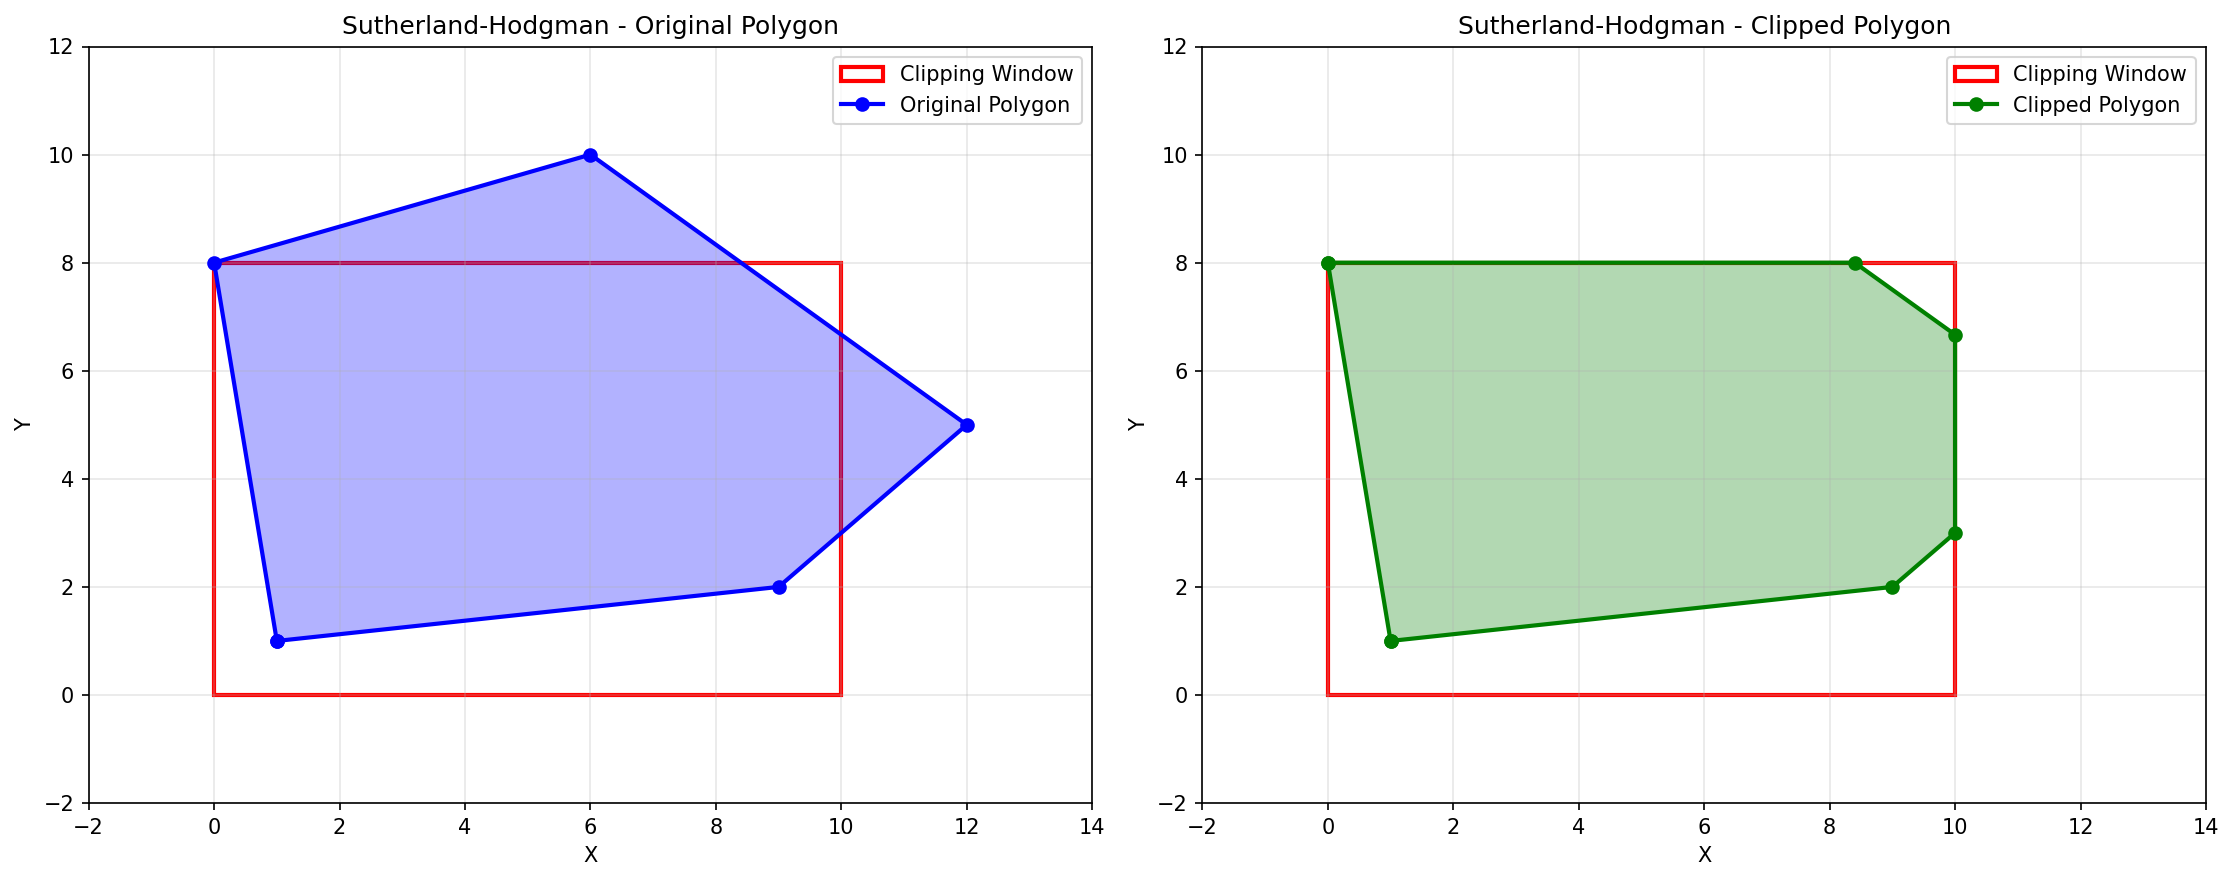
\includegraphics[width=0.8\textwidth]{output_sutherland_hodgman.png}
    \caption{Sutherland-Hodgman: Original polygon vs Clipped polygon against rectangular window}
\end{figure}

\newpage
%===========================================
% CONCLUSION
%===========================================
\section{Conclusion}

This laboratory exercise provided comprehensive hands-on experience with fundamental clipping algorithms in computer graphics. The three clipping algorithms implemented demonstrate different approaches to solving visibility problems in 2D graphics.

\textbf{Key Learnings:}
\begin{itemize}
    \item \textbf{Cohen-Sutherland Algorithm:} Uses region codes and divide-and-conquer approach for line clipping, efficient for cases where many lines are completely inside or outside
    \item \textbf{Liang-Barsky Algorithm:} Uses parametric line representation for more efficient calculations, particularly effective for lines that intersect the clipping window
    \item \textbf{Sutherland-Hodgman Algorithm:} Handles polygon clipping through successive edge clipping, works for any convex clipping window
    \item \textbf{Clipping Windows:} Understanding the mathematical representation of boundaries and intersection calculations
    \item \textbf{Geometric Computations:} Line-line intersection, point-in-polygon tests, and parametric representations
    \item \textbf{Region Codes:} Binary encoding of spatial relationships for efficient visibility testing
\end{itemize}

\textbf{Technical Insights:}
\begin{itemize}
    \item Understanding the mathematical foundation of computational geometry in graphics
    \item The importance of efficient algorithms for real-time graphics applications
    \item How different algorithms excel in different scenarios (line density, intersection frequency)
    \item The relationship between clipping and rendering pipeline optimization
    \item Parametric vs. implicit representations and their computational trade-offs
    \item The significance of convexity assumptions in algorithm design
\end{itemize}

\textbf{Observations:}
\begin{itemize}
    \item Cohen-Sutherland is conceptually simple but may require multiple iterations for lines crossing multiple boundaries
    \item Liang-Barsky provides more efficient computation through parametric approach and single-pass processing
    \item Sutherland-Hodgman elegantly handles complex polygon clipping through iterative edge processing
    \item All algorithms maintain geometric accuracy while providing computational efficiency
    \item Proper handling of edge cases (parallel lines, degenerate polygons) is crucial for robust implementation
    \item These clipping algorithms form essential components of graphics rendering pipelines
\end{itemize}

The laboratory exercise successfully demonstrated how mathematical geometric concepts translate into practical clipping solutions. Understanding these fundamental algorithms provides essential knowledge for graphics programming, CAD systems, game development, and visualization applications where efficient visibility determination is crucial.

\end{document}